\section{Monte Carlo and data comparison}
\label{app:MC_data_comp}

In these appendix we report a comparison between distributions of variables in data and MC.
This plots where used to understand which variables have good discriminating power and to check for
data-MC discrepancies.


In the plots what is labeled "Data" is real data %in a 20 MeV interval around the \Lb mass,
where we use the sideband subtraction technique to remove background.
"Side" is real data for masses above 5.4 GeV containing mostly combinatorial background.
This can be compared to the previous sample to see which variables differ most in signal and background events.
 
"MC" is Pythia 8 \Bz\to\Kstar\jpsi fully weighted MC, where we don't ask for the true ID of reconstructed particles.

Distributions are shown separately for the electron and muon channels.


\begin{figure}[h!]
\centering
\includegraphics[width=0.48\textwidth]{RKst/figs/MC_data_comp/EE/drawVariables_B0_DTF_PV_chi2_B0_DTF_PV_nDOF.pdf}
\includegraphics[width=0.48\textwidth]{RKst/figs/MC_data_comp/MM/drawVariables_B0_DTF_PV_chi2_B0_DTF_PV_nDOF.pdf}
\caption{ Distributions of the $\chi^2/ndf$ of the kinematic fit in MC, data signal and data background for electron (left) and muon (right) channles.   }
\end{figure}

\begin{figure}[h!]
\centering
\includegraphics[width=0.48\textwidth]{RKst/figs/MC_data_comp/EE/drawVariables_B0_P.pdf}
\includegraphics[width=0.48\textwidth]{RKst/figs/MC_data_comp/MM/drawVariables_B0_P.pdf}
\caption{ Distributions of \Bz momentum in MC, data signal and data background for electron (left) and muon (right) channles.   }
\end{figure}

\begin{figure}[h!]
\centering
\includegraphics[width=0.48\textwidth]{RKst/figs/MC_data_comp/EE/drawVariables_B0_PT.pdf}
\includegraphics[width=0.48\textwidth]{RKst/figs/MC_data_comp/MM/drawVariables_B0_PT.pdf}
\caption{ Distributions of the $\chi^2/ndf$ of the kinematic fit in MC, data signal and data background for electron (left) and muon (right) channles.   }
\end{figure}

\begin{figure}[h!]
\centering
\includegraphics[width=0.48\textwidth]{RKst/figs/MC_data_comp/EE/drawVariables_B0_DIRA_OWNPV.pdf}
\includegraphics[width=0.48\textwidth]{RKst/figs/MC_data_comp/MM/drawVariables_B0_DIRA_OWNPV.pdf}
\caption{ Distributions of \Bz transverse momentum in MC, data signal and data background for electron (left) and muon (right) channles.   }
\end{figure}

\begin{figure}[h!]
\centering
\includegraphics[width=0.48\textwidth]{RKst/figs/MC_data_comp/EE/drawVariables_B0_FDCHI2_OWNPV.pdf}
\includegraphics[width=0.48\textwidth]{RKst/figs/MC_data_comp/MM/drawVariables_B0_FDCHI2_OWNPV.pdf}
\caption{ Distributions of the $\chi^2/ndf$ of the kinematic fit in MC, data signal and data background for electron (left) and muon (right) channles.   }
\end{figure}


\begin{figure}[h!]
\centering
\includegraphics[width=0.48\textwidth]{RKst/figs/MC_data_comp/EE/drawVariables_B0_ENDVERTEX_CHI2_B0_ENDVERTEX_NDOF.pdf}
\includegraphics[width=0.48\textwidth]{RKst/figs/MC_data_comp/MM/drawVariables_B0_ENDVERTEX_CHI2_B0_ENDVERTEX_NDOF.pdf}
\caption{ Distributions of the $\chi^2/ndf$ of the \Bz decay vertex quality in MC, data signal and data background for electron (left) and muon (right) channles.   }
\end{figure}



\begin{figure}[h!]
\centering
\includegraphics[width=0.48\textwidth]{RKst/figs/MC_data_comp/EE/drawVariables_Kst_PT.pdf}
\includegraphics[width=0.48\textwidth]{RKst/figs/MC_data_comp/MM/drawVariables_Kst_PT.pdf}
\caption{ Distributions of \Kstar transverse momentum in MC, data signal and data background for electron (left) and muon (right) channles.   }
\end{figure}

\begin{figure}[h!]
\centering
\includegraphics[width=0.48\textwidth]{RKst/figs/MC_data_comp/EE/drawVariables_Kst_IPCHI2_OWNPV.pdf}
\includegraphics[width=0.48\textwidth]{RKst/figs/MC_data_comp/MM/drawVariables_Kst_IPCHI2_OWNPV.pdf}
\caption{ Distributions of \Kstar $IP\chi^2$ in MC, data signal and data background for electron (left) and muon (right) channles.   }
\end{figure}

\begin{figure}[h!]
\centering
\includegraphics[width=0.48\textwidth]{RKst/figs/MC_data_comp/EE/drawVariables_Kst_ENDVERTEX_CHI2_Kst_ENDVERTEX_NDOF.pdf}
\includegraphics[width=0.48\textwidth]{RKst/figs/MC_data_comp/MM/drawVariables_Kst_ENDVERTEX_CHI2_Kst_ENDVERTEX_NDOF.pdf}
\caption{ Distributions of the $\chi^2/ndf$ of the \Kstar decay vertex quality fit in MC, data signal and data background for electron (left) and muon (right) channles.   }
\end{figure}








